% Chapter 3

\chapter{WiSARDNet Cyberinfrastructure} % Write in your own chapter title
\label{Chapter 3}
\lhead{} % Write in your own chapter title to set the page header

\section{Overview}
This chapter describes the platform on which the work of this thesis is built. WiSARDNet is a WSN platform which consists of hardware and software that connect sensor/actuator nodes to users. The National Science Foundation has adopted the term cyberinfrastructure to describe computational systems with advanced data acquisition, processing, and management capabilities. According to this definition, WiSARDNet can be thought of as cyberinfrastructure. Each network component is described in this chapter, as well as the data management and archival processes. The cyberinfrastructure hardware and software components can be divided into four categories: WSN, base station, real-time data center (RTDC), and end-user. Figure \ref{fig:device_hierarchy} shows how the hardware and software components for each of these categories fit together. The core component which links the WSN, the base station, and the real-time data center is a TCP/IP based message broker that uses the MQTT protocol. MQTT will be described in further detail in this chapter. Additionally, database archival components will be described in terms of their role in the cyberinfrastructure in this chapter. The technical specifics of the database from a software perspective will be described in greater detail in Chapter 4.

\begin{figure}[htbp]
	\centering
	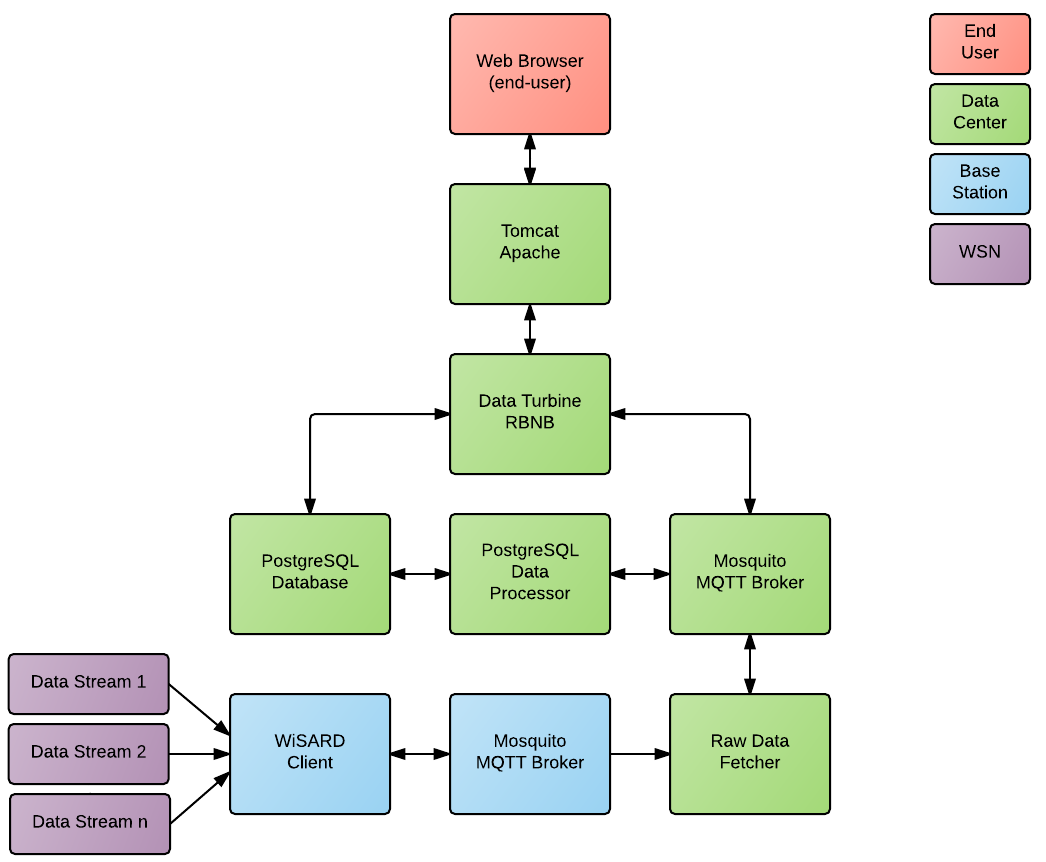
\includegraphics[width=\textwidth]{figures/WiSARDNet_architecture.png}
	\caption{Cyberinfrastructure hardware and software component hierarchy}
	\label{fig:device_hierarchy}
\end{figure}

\section{WiSARD Devices}
The Wireless Sensing and Relay Device (WiSARD) is a sensor/actuator (S/A)  device designed to be modular, adapting easily to the different sensing and actuation needs of users. Flexibility and energy awareness are the two driving design motivations in the WiSARD development. At the heart of each WiSARD device is a central processor (CP) which governs the operation of the device and its peripherals. The CP dictates when and how tasks will be scheduled and executed, establishes and manages wireless links to other WiSARDs, facilitates the storage of sensor readings, and offloads the sensing and actuation tasks to daughterboards called satellite processors (SP). A WiSARD can accommodate up to four different SPs. This enables each WiSARD to perform a variety of tasks specifically tailored to meet the needs of researchers and experimenters. The modular design allows the CP to offload sensing operations to its SPs which can execute tasks in parallel with CP operation. 

Both CP and SP boards use an MSP430 16-bit ultra-low-power microcontroller by Texas Instruments. This microcontroller has a variety of features and also allows for the device to be placed in various low-power modes. The low-power modes of operation accompanied by energy conscious software design allow for a WiSARD to operate on a single pack of AAA batteries for many weeks or even months, depending on the rate at which the devices dispatch their sampling operations. The CP also connects to a radio board which uses an Analog Devices ADF7020 RF transceiver module that operates in the 902-928 MHz license-free ISM band.  When WiSARDs are powered up, they autonomously form a self-organizing and self-healing multi-hop wireless ad-hoc network. A special WiSARD which is assigned the software role of Hub acts as the base station, and is connected to an embedded Linux computer referred to as a garden server. 

\section{Middleware}

%The central architectural component which connects the garden servers to the RTDC is an open-source data streaming middleware software named Data Turbine. Data Turbine can be thought of as a data streaming engine acting as a ring-bufferred network bus (RBNB) which is a versatile and portable data streaming solution. Middleware software solutions operate under one of two operational paradigms: request/response or publish/subscribe. RBNB is a data broker which operates under the request/response paradigm of middleware software.  From an architectural standpoint, there are 3 core components to a Data Turbine implementation: servers, sources, and sinks. The Data Turbine server houses the actual data structure which manages the data and makes it available for request. Data Turbine Source objects aggregate data for insertion into the Data Turbine server. Alternatively, Data Turbine sink objects request data from the Data Turbine server and make it available to the process or user that desires it. Data turbine was written in Java, and is therefore versatile in the number of platforms upon which servers, sources, and sinks can execute. This, as well as the Data Turbine application programming interface (API) allows for a variety of data-centric applications and experiments to be performed. 

Middleware is a term which describes a software abstraction of the transfer of information from point A to  point B. By hiding the complexities of data transport behind a simple interface that connects two pieces of software, the development of powerful data processing and management tools can be accelerated. WiSARDNet relies heavily upon the use of middlware to make the WSN data available to the rest of the world.\\

The central architectural component that connects the garden servers to the RTDC is MQTT. MQTT is a data transfer protocol created by IBM that utilizes the publish/subscribe middleware paradigm. An MQTT broker can be installed on a computer or server and will then listen for TCP/IP connection requests. A data source on another device can publish data by connecting to the broker and sending data messages. WiSARDNet uses Mosquitto~\cite{mosquitto}, an open source implementation of a message broker that uses the MQTT protocol.\\ 

A message broker installed on each garden server keeps all of the data from that site in persistent storage, which is a collection of archived data files on the hard disk. To transfer the data from the WiSARDs to the broker, a Java application referred to in WiSARDNet as a WiSARD client uses MQTT messages to publish data. The RTDC can then retrieve all of the data with a subscription client by connecting to the garden server's message brokers over cellular or satellite connections.\\

An MQTT subscription client for each garden site run at the RTDC and is responsible for subscribing to all the data published to each broker. These subscription clients are what is referred to in WiSARDNet as a raw data fetcher (RDF).  The purpose of the RDFs is to retrieve all of the data from all of the gardens so that the data is accessible for processing, storage, or viewing. These processes are discussed in detail in the following section.\\

%Within the WiSARDNet CI, each garden server runs a local instance of the Data Turbine server. Data Turbine Source objects are small software programs which funnel data gathered from the local WiSARD network feed data into the Data Turbine server. Alternatively, sink objects pull data out of the Data Turbine server. Data Turbine uses what is referred to as a channel map as a means to associate individual data channels with the Data Turbine streams that connect sources and sinks to the Data Turbine server. At the RTDC, a much larger instance of the Data Turbine server runs, with source objects connecting to each garden server. By initializing a Data Turbine sink, a user or application may request specifically identified data channels from the Data Turbine server using a channel map with the names defined by the user in the source. In the WiSARDNet CI, the Data Turbine server at the RTDC requests all new data at regular intervals from the Data Turbine server instances at each garden, and inserts the data into a single central location. These requests are made via TCP/IP connections between the garden servers and the RTDC via their cellular or satellite based Internet connections. The WiSARDs themselves are not directly ip-addressable and therefore funneling data to the RTDC via each garden's base station greatly simplifies the procedure of requesting data from each location.

\section{Real-time Data Center}
The RTDC is a collection of servers which host a Tomcat Apache web server, a Mosquitto MQTT subscription client, an instance of an open-source data streaming middleware called Data Turbine, a PostgreSQL relational database, and all of the data management processes and applications which interact with the WSN. The RTDC has several functions, the first of which is to retrieve all of the WSN data from each of the gardens. The RTDC is a centralized destination for all of the network's data streams. From this location, applications can access, store, and modify data for their various needs, as opposed to having to interact with multiple networks individually. For instance, a process which reads in raw data streams from temperature sensors might need to calculate human-readable values from the raw sensor readings, such as degrees Celsius. A single data converting processor which moves data from raw transducer values to human-readable values, can easily acquire all of the raw data streams for temperature sensors at all network locations with a single fetch, rather than requiring that the process fetch the raw data from each specific garden individually. Additionally, aggregating all data at the RTDC greatly simplifies archival and backup procedures.\\

\subsection{Relational Database}
Relational databases provide a flexible way to store and access large amounts of data. A relational database is composed of one or more tables; tables are 2 dimensional matrices of rows and columns. According to Rockoff ~\cite{rockoff2010language}, rows and columns are referred to as records and fields, respectively. An entry in a database table occupies a single row and each field corresponding to a different attribute of that entry constitutes a new column. For example, a table which stores people might have columns for an identification number, a name, an address, and a telephone number. An entry of a new person into this table would occupy a single row, with the data matching each of the attributes would occupy the rows' intersections with each column. Formally, these columns are referred to as primary keys, as they map individual fields to the entries which they belong. The database at the RTDC has numerous tables which store information about every device, every garden location, and the sensor readings themselves.\\ 

In WiSARDNet, data streams are archived in a PostgreSQL table. Additional tables in this database store all of the meta-data and logistical information regarding all of the WSN devices, as well as every data point sampled from any of the gardens. Additionally, there are many data streams that also need to be tracked and archived such as diagnostic control data, error reporting, and other useful information that help with network upkeep. An example of diagnostic control data might be the logging of a device restart event; such events can be crucial in detecting and analyzing network performance issues.\\

At the RTDC, the PostgreSQL database is physically located on its own server, separate from the other data management and processing clients. By placing the database on a separate server, the database has exclusive access to dedicated processing resources to allow for the quickest possible query and insert response times for the the data schema and the queries used. Another function that the RTDC performs is the execution of applications and processes which interact with the WSNs and their data. One example of an application running on a server at the RTDC might be a researcher performing an experiment which attempts to maintain equal soil moisture readings at two different geographic locations. The RTDC servers possess high-performance computing hardware such that many applications and processes can use to interact  with the networks in real-time. By executing these applications and processes at the RTDC, they will operate at optimal performance, minimizing latency from performing queries and calculations to preserve as close to a real-time experience as possible.

\subsection{Data Schema}
WiSARD hardware components are subject to a design hierarchy which specifies how the different pieces organize and interact in operation. Figure \ref{fig:device_hierarchy_edit} shows the hierarchy of the WiSARD hardware components. 

\begin{figure}[htbp]
	\centering
	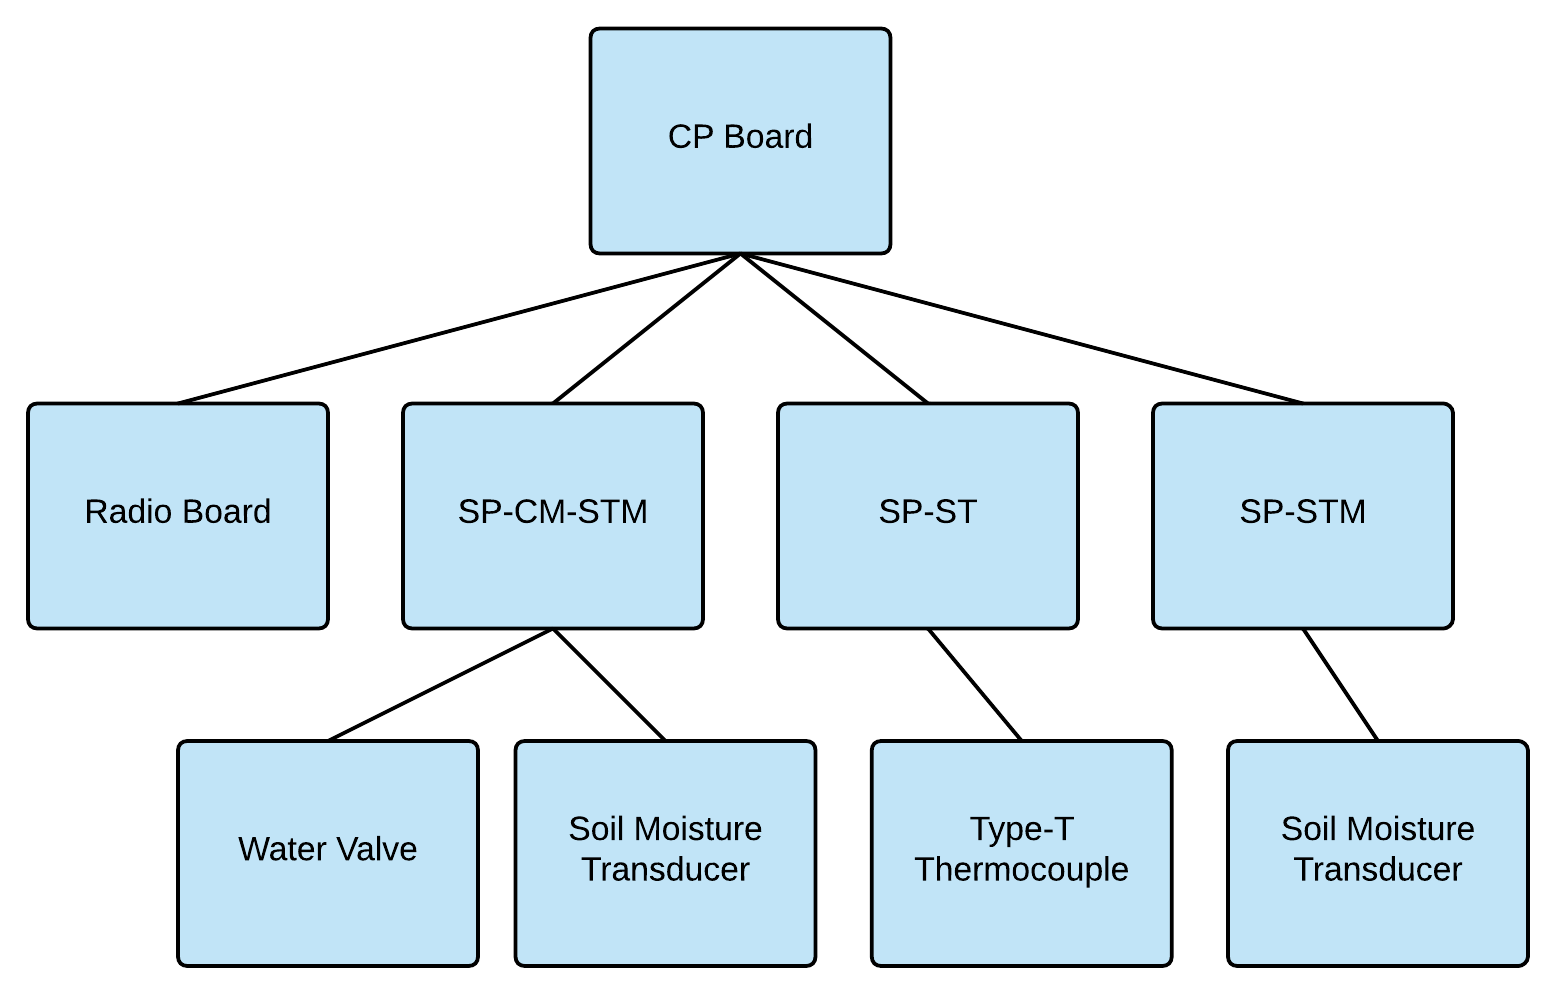
\includegraphics[width=\textwidth]{figures/wisard_device_hierarchy.png}
	\caption{Device Relationship Structure}
	\label{fig:device_hierarchy_edit}
\end{figure}

In a similar manner, the data gathered in WiSARDNet follows a design hierarchy that specifies how data is organized. The organizational structure of the the data tables and their relations, or the data schema as it is commonly referred to, was specifically designed to best accommodate the ever-changing configuration status of WiSARDNet devices. Every piece of hardware is referred to in the data schema as a device, and therefore the primary table in the data schema is the Device table. A record in the device table will describe any device of any type. For instance, a radio, a soil-moisture transducer, a satellite processor, or a garden server are all devices that have a record in the device table. The configuration of these devices, however, might change at some point in time; it might be moved to another location, it might be upgraded or replaced, or it might receive a new firmware version. In this schema, the device's software parameters, hardware configuration, and state of operation are all encapsulated in a Deployment. Using the hierarchical structure of the WiSARD hardware, we use a tree structure in grouping devices together through their deployment records. Figure \ref{fig:deployment_hierarchy_edit} shows how devices and deployments are structured in the database. Each deployment record has a field for a parent device deployment. 

\begin{figure}[htbp]
	\centering
	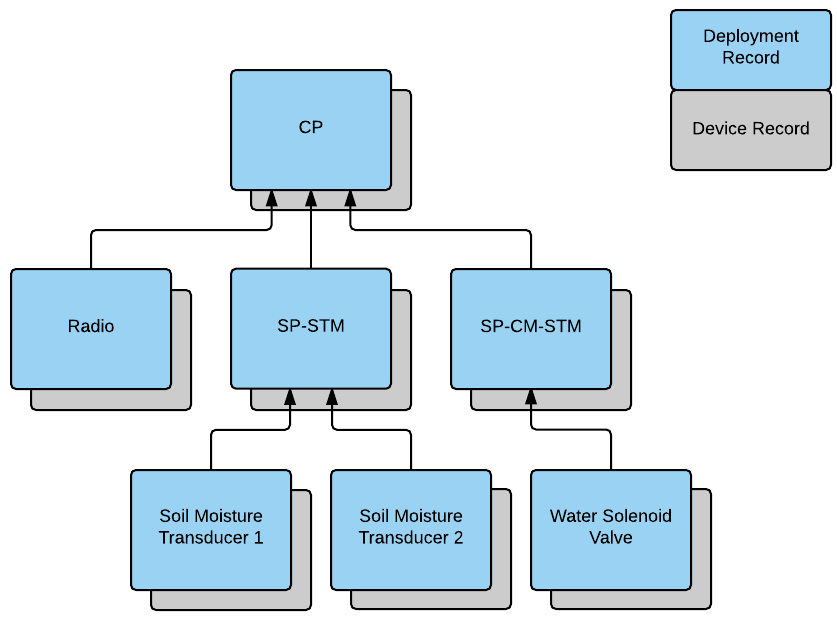
\includegraphics[width=\textwidth]{figures/deployment_hierarchy_edit.png}
	\caption{Deployment Relationship Structure}
	\label{fig:deployment_hierarchy_edit}
\end{figure}

If a particular transducer is attached to a satellite processor, then its active deployment record references the satellite processor's deployment record in the parent deployment field. These are recorded and tracked through a deployment table where each record is a particular deployment that references a device record in the device table. When a change is made to any of the parameters tracked in the deployment table, the device is thought of as having a new deployment, and therefore a new record is inserted into the deployment table, and the device record is referenced by the new deployment. The key field in the deployment table is a binary field which stores a true/false value of whether or not the deployment is active. Once a deployment is changed, the old deployment becomes inactive and the new deployment becomes active. Over time, many deployment records may accumulate for a particular device as changes are made; the entire history of the device is stored so that for any given data point, the deployment configuration of the device associated with that data sample is accessible.\\

Having the ability to store and track each device's configuration and related meta data in the database is of great value in the management of the networks and the various experiments. When a WiSARD is ready for deployment at a garden site, a deployment record is created with all of its configuration data, the deployment record is set to active, and the start date and time is set. As long as the device remains in this configuration, the deployment object pointing to that device will remain active. If a setting changes or if a sensor fails and is replaced for instance, the following actions are taken:

\begin{enumerate}
	\item The deployment record to which the failed sensor device points is set to inactive.
	\item The current time is inserted into the stop-time field of the deployment record 
	\item The replacement sensor is added as a record to the device table
	\item A new deployment record is inserted into the deployment table
	\item The parent field of the new deployment record references the deployment record of the SP device to which it is installed
	\item The active status field of the new deployment record is set to active
	\item The current time is inserted into the start-time field of the new deployment record
\end{enumerate}

By following this procedure, previous device configurations are current configurations are easily accessible from the database as well as any previous configurations and the the time period which the were active. Active and inactive deployment tracking through a single record addition for each instance of a configuration change is trivial with regards to computational complexity and storage resources. This approach is simple, intuitive, and scales well as the number of devices deployed in the field increase. With this system in place for accessing up-to-date configurations of any registered device, there is now a foundation in place for fully describing every single data point which is sampled from any transducer or device. With this paradigm, a data sample is not merely a sample from a device,  it is a sample from a specific deployment of a device. When a device's configuration is altered, producing a new deployment for that device, the data generated by that device becomes a new stream.\\

When new data from WiSARDs arrive at the RTDC from the MQTT broker, they need to be accessible for users and other services to request. Data Turbine's network accessible ring buffer data structure works well for this purpose. At the RTDC, the data streams arriving via MQTT are placed into Data Turbine's ring buffer in accordance with the stream name which identifies the device from which the sample was taken. Since the complexities of WiSARD configurations are handled via the device, devicetype, and deployment tables, archival of sampled data in the database becomes a simple procedure. All samples from all streams are placed as individual records in a table named data. In addition to the sampled value and the time at which it was sampled, the sample via its Data Turbine stream name can be mapped to the specific device and deployment records for which the deployment was active. In this way, data archival of acquired samples is extremely simple and all information regarding a device and its samples is easily accessible and intuitively obtained through the thoughtful design of the data schema. 

\section{Summary}
WiSARDNet is a WSN CI which was designed from the ground up to be modular, scalable, and accessible to users. The Mosquitto MQTT broker, the data streaming middleware Data Turbine, and the RTDC enable data sampled from sensors to be retrieved, managed, processed, and archived into a PostgreSQL database. The way in which WiSARD meta-data and configuration information is stored and accessed is critical for the development of a network configuration software which comprises the work of this thesis. How these features are utilized in the network management software is described in further detail in Chapter 4.